I have tabulated the following TODO list.

\begin{enumerate}
  \item 
    Learn to convert gigatons of carbon to parts per million in the atmosphere.
    \begin{enumerate}
      \item Parts per million by volume and parts per million by mass. Conversion ratio of molar mass of C by molar mass of CO$_2$.
      \item Note that the ppm of carbon emissions is changing annually. Currently, the value is 400 ppm.
      \item 
        Resource \path{https://micpohling.wordpress.com/2007/03/30/math-how-much-co2-by-weight-in-the-atmosphere/}
    \end{enumerate}
  \item Read the manuscript ~\citet{DR:2013}
  \item Research the carbon fluctuations in the atmosphere during the phenozoric period. 
    \begin{enumerate}
      \item Analyze the following plots:
        \begin{enumerate}
          \item 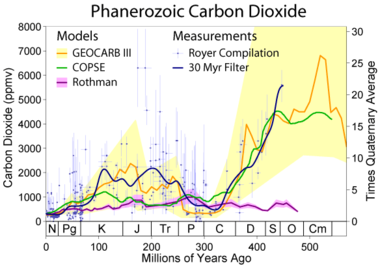
\includegraphics[scale=0.5]{00LOG/UNDATED/00FIGURES/Phanerozoic_Carbon_Dioxide.png}
          \item 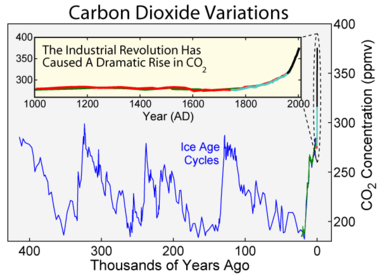
\includegraphics[scale=0.5]{00LOG/UNDATED/00FIGURES/Carbon_Dioxide_400kyr.png}
          \item 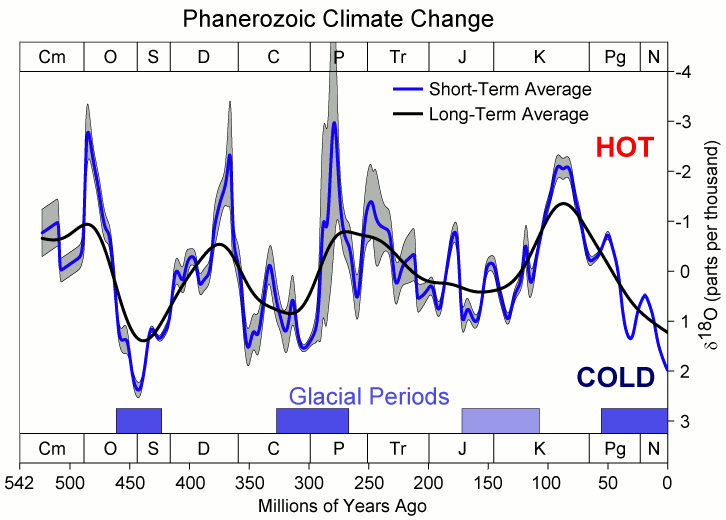
\includegraphics[scale=0.25]{00LOG/UNDATED/00FIGURES/Phanerozoic_Climate_Change.png}
        \end{enumerate}
      \item Understand how the measurements are being made in terms of temperature, ~\ce{CO2}, etc.
      \item Reference \path{https://en.wikipedia.org/wiki/Carbon_dioxide_in_Earth\%27s_atmosphere}.
    \end{enumerate}

  \item Read the paper ~\citet{RDL:2014}. 
    \begin{enumerate}
      \item Status: Start reading up to 6.11.2.2 GEOCARB Models as of 1156 PDT 3/28/17
      \item Questions:
        \begin{enumerate} 
          \item What, who and how did GEOCARBB model come to be?         
          \item Are \ce{CaSiO3} and \ce{MgSiO3} metamorphic rocks?
          \item the weathering of \ce{Ca^{2+}} and \ce{Mg^{2+}} silicate rocks consumes a stoichiometrically equivalent amount of \ce{CO2}. Stoichiometrically equivalent??
        \end{enumerate}
     \item Notes:
        \begin{enumerate}
          \item Carbonic acid is chemically written as \ce{HCO3^-}. 
          \item \ce{Ca^{2+}}, \ce{Mg^{2+}} ions are derived from \ce{CaSiO3} and \ce{MgSiO3} reacting with \ce{HCO2^-}.
          \item Weathering of calcium silicates, one major \ce{CO2} sink is chemically written as \\
          \begin{eqnarray}
            \ce{2CO2 + H2O + CaSiO3 -> Ca^{2+} + SiO2 + 2HCO3^-} \\
            \ce{Ca^{2+} + 2HCO3^- -> CaCO3 + CO2 + H2O} 
          \end{eqnarray}
          
          and adding the two equations gives us

          \begin{equation}
            \ce{CO2 + CaSiO3 -> CaCO3 + SiO2}
          \end{equation}
     
          Notice that, Carbonate formation releases a stoichiometrically equivalent amount of \ce{CO2} , but the weathering of one mole of silicate mineral consumes two moles of \ce{HCO3^-}. The weathering of \ce{Ca^{2+}} and \ce{Mg^{2+}} silicate rocks consumes a stoichiometrically equivalent amount of \ce{CO2}.
      		   
          In this Treatise, the identification of these processes are attributed to French chemist and mining engineer J.J. Ebelmen in 1845. Urey is credited with a more modern treatment in 1952.

          \item The second major \ce{CO2} sink is the burial of organic material on land (or in the ocean). Physcial seperation of buried \ce{CH2O} is released ten to 100 million years as a result of plate tectonic forces either through degassing, or chemical weathering adding \ce{C} into the atmosphere. Coined as geo-respiration. The inverse process of burial is coined as geo-photosynthesis. The chemical equation is written as
          \begin{equation}
            \ce{CO2 + H2O -> CH2O + O2}
          \end{equation}

          \item \ce{CO2} and \ce{O2} are decoupled because the processes that influence these quantities in the atmosphere are independent of each other.
          \item The short term carbon cycle influences the atmosphere on time scales of thousands of years. The components that influence the short term carbon cycle can be decoupled for the components that influence the long term carbon cycle. Short term carbon cycle determines the fluxes of carbon in the surface reservoirs.  
          \item Long term carbon cycle is influenced by its constitutive bells and whistles on the time scale of > $10^5$ years.   
        \end{enumerate}
    \end{enumerate}    
\end{enumerate}
